
\section{Robustness Metrics}
\label{sec:sensitivity}


Many computational scientists develop and use large-scale, loosely-coupled applications that are often structured as scientific workflows, which consist of many computational tasks with data dependencies between them. When executing these applications on a multi-machine distributed environment, such as the Grid or the Cloud, significant system overheads may exist~\cite{Chen2011, Prodan2008, Dong2010, Yang03, Chen2012a} and the problem of choosing robust schedules becomes more and more important. Traditionally, a carefully crafted schedule is based on deterministic or statistic estimates for the execution time of computational activities that compose a workflow. However, in such an environment, this approach may prove to be grossly inefficient~\cite{Chen2012a}, as a result of various unpredictable overheads that may occur at runtime. 
%Particularly, it is challenging to provide a good estimate of overheads since it involves a lot of uncertainties. 
Thus, to mitigate the impact of uncertain overheads, it is necessary to choose a schedule that guarantees overhead robustness, that is, a schedule that is affected as little as possible by various overhead changes.  

There are several ways to achieve overhead robustness. A first approach is to integrate the overhead estimation into the job scheduling problem. A static or statistic estimation of communication cost or data transfer delay~\cite{Dong2010, Yang03} has been considered in the scheduling problem. Once we have the deterministic or statistic information of overheads, we can treat the system overhead as computational activities and the goal is to minimize the overall runtime including overhead duration. However, this approach only applies to the estimation of data transfer delay since the highly unpredictable variability and variety of other overheads make it a challenging work and not efficient in practice. Our prior work~\cite{Chen2011} has shown the variation of overheads may be comparable to the job runtime and thus makes it unrealistic in a real environment.  

A significant amount of work~\cite{Chetto1990, Dong2010, Yang03} in the literature has focused on proposing algorithms that are aware of the dynamic changes of runtime environments. Task rescheduling~\cite{Sakellariou2004, Zhang2009a} is a typical approach that dynamically allocates tasks to an idle processor in order to take into account information that has been made available during the execution. Specifically, resource load~\cite{Dong2010} can be used to estimate the variance. However, rescheduling a task is costly as it implies some extra communication and synchronization costs. Relevant studies~\cite{Sakellariou2004} indicate that it is important to have a static schedule with good properties before the start of the execution. Therefore, even if a dynamic strategy is used, a good initial placement would reduce the possibility of making a bad decision. 

Another approach is to overestimate the execution time of individual jobs. Delay scheduling~\cite{Zaharia2010} waits for a small amount of time, letting other MapReduce jobs launch tasks instead and this method can achieve a better tradeoff of locality and fairness. However, this method only applies to workload scheduling and particularly MapReduce jobs since the duration of them is short and thus it is not difficult to estimate the scheduling delay. Also, this results in a waste of resources as it induces a lot of idle time during the execution, if the overhead is shorter than the estimation. Second, overheads do not simply work as an attachment to the job runtime and it involves a lot more complicated patterns such as periodicity~\cite{Chen2011}. 

In this section, we first present our work on evaluating the overhead robustness of scheduling heuristics and we indicate a list of structural heuristics that are overhead robust. Second, since the estimate of overhead duration is difficult, we develop new heuristics that leverage the pattern information of workflow overheads, which represents a new approach to design overhead robust algorithms. To the best of our knowledge, so far, no study has systematically tried to evaluate the scheduling heuristics with respect to the overhead robustness.  



\subsection{Overhead Patterns}

In this section, we introduce the common overhead patterns in workflow execution. 
In scientific workflow systems, time related functionalities such as workflow scheduling normally requires effective forecasting of activity patterns. In this work, we mainly focus on the overhead pattern that refers to a representative time series of overhead activities that occurs repeatedly and regularly in workflow execution. An overhead pattern is composed of ordered overhead activities obtained from scientific workflow system logs or other forms of historical data. 
Pattern discovery~\cite{Liu2008} usually starts from a periodical sampling plan to build representative duration series (Job Release, etc. ) and then conducts time-series segmentation to discover the pattern sets and predicts the activity duration intervals with pattern matching results. 


The motivation for pattern based analysis comes from the observation that for those duration-series segments where the number of concurrent activity instances is similar, these activity durations reveal comparable statistical features. Due to the dynamic nature of underlying resources, pattern based forecasting of overheads can improve the effectiveness of scheduling heuristics. 

\begin{figure}[htb]
\centering
 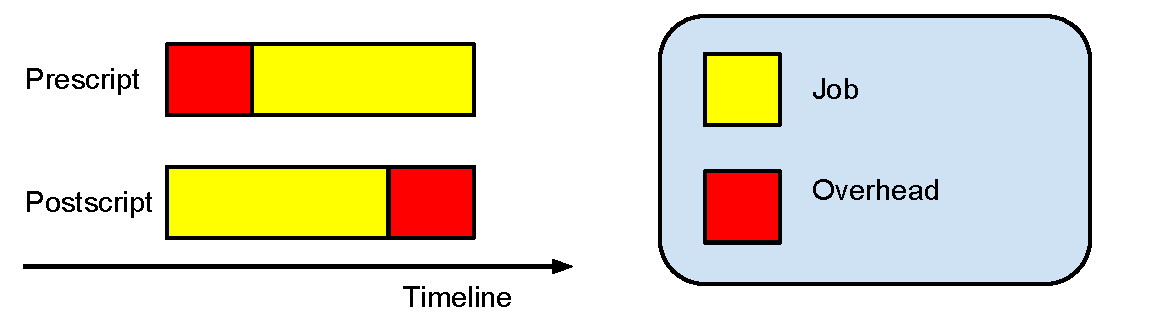
\includegraphics[width=1\linewidth]{figures/sensitivity/adherence.pdf}
  \captionof{figure}{Adherence Pattern}
  \label{fig:sensitivity_adhere}
\end{figure}

Most of the work~\cite{Dong2010, Yang03} view the overhead duration as an attachment to runtime in workflow timeline. For example, the Pre/Post-script Delay is usually constant, which we call it Adherence Pattern as shown in Fig.~\ref{fig:sensitivity_adhere}. Scheduling algorithms can just add the delay to the job runtime without significant change to the algorithms. For this pattern, we have shown in our prior work~\cite{Chen2012a} that it does not have much influence on the overhead robustness. 
However, we observe that the Workflow Engine Delay and the Queue Delay increases periodically and steadily. For example, Fig.~\ref{fig:sensitivity_trace} shows the Gantt chart of part of a real trace\footnote{Details: http://www.isi.edu/\string~wchen/fgrid/run}. 
The Workflow Engine Delay (red) of the first 16 jobs is 5 seconds and then it increases to 10 seconds. 
%It is difficult to explain queue delay
We call this common overhead pattern the Incremental and Periodical Pattern (IPP). We observe the Queue Delay also increases periodically but the period is interrupted by the resource availability and thus it has a more complicated IPP. In the rest of this paper, we focus on the IPP of the Workflow Engine Delay and we will cover the Queue Delay in our future work. 
The reason why IPP prevalently exists is that many workflow management components are queue based systems. They repeatedly check their queues to find whether there are idle jobs, if yes they will process and submit these jobs, otherwise it will wait for a interval and continue. In Fig.~\ref{fig:sensitivity_ipp} we abstract the IPP from the trace, which shows a repeatedly increase by a interval. We define throughput of a workflow management component as the maximum number of allowed jobs in queue. For example, the interval and the throughput of the Workflow Engine in Fig.~\ref{fig:sensitivity_trace} are around 5 seconds and 16 respectively. 


\begin{figure}[htb]
\centering
 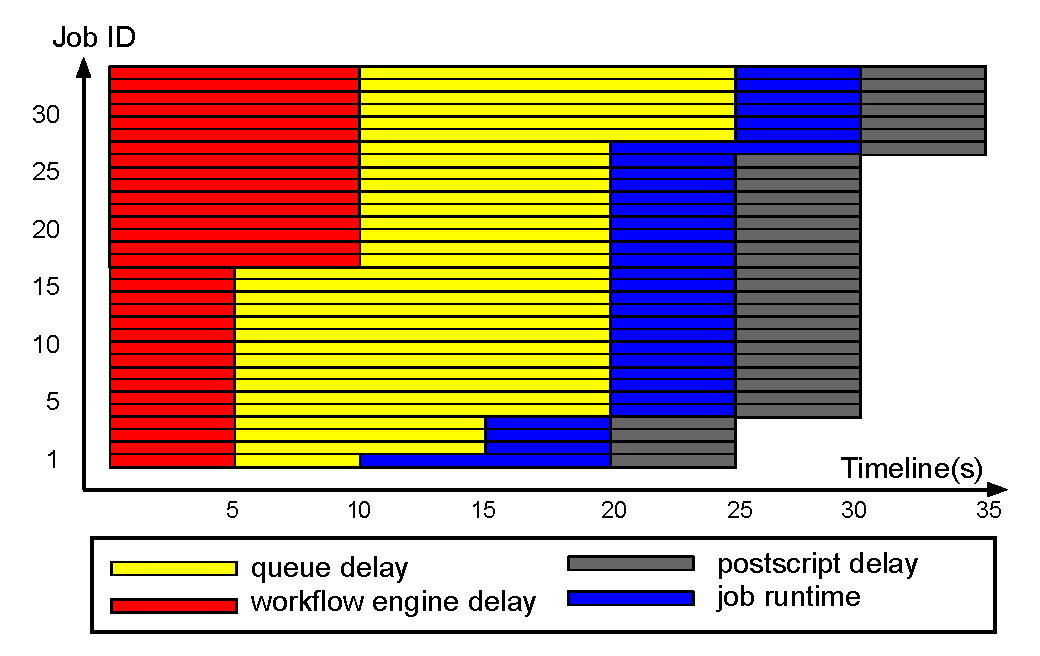
\includegraphics[width=1\linewidth]{figures/sensitivity/trace.pdf}
  \captionof{figure}{Workflow Execution Gantt Chart of a Real Trace}
  \label{fig:sensitivity_trace}
\end{figure}


These overhead patterns reappear frequently during a duration series and they represent unique behavior of the workflow management components. After we define and discover these typical patterns, the intervals and throughputs of these patterns can be estimated and statistically captured from historical traces. 


\begin{figure}[htb]
\centering
 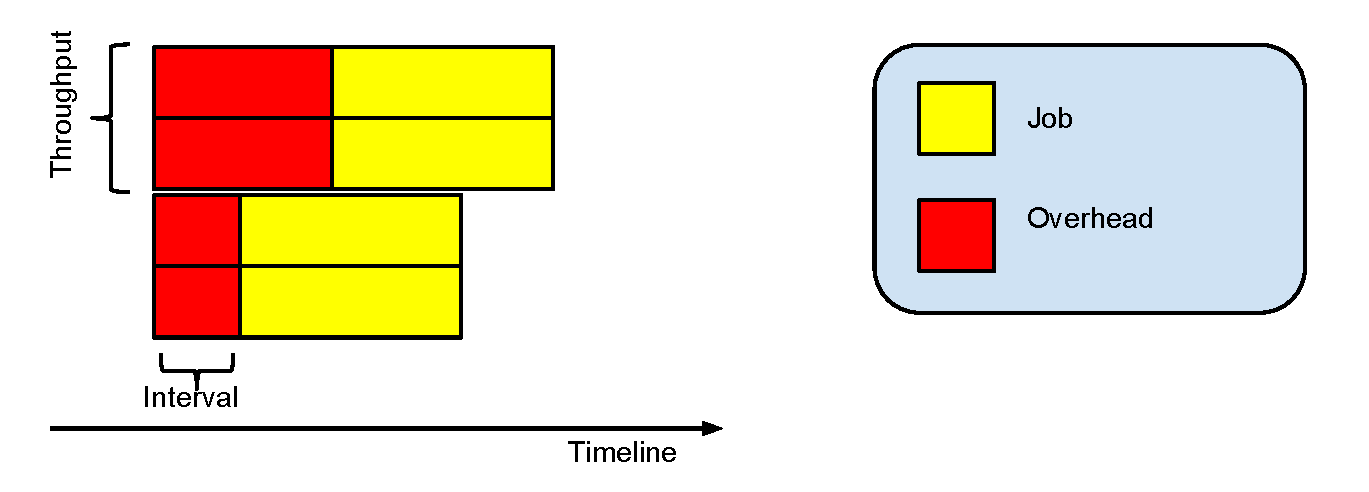
\includegraphics[width=1\linewidth]{figures/sensitivity/incremental.pdf}
  \captionof{figure}{Incremental and Periodical Pattern}
  \label{fig:sensitivity_ipp}
\end{figure}

%It is not workflow engine delay it is workflow engine interval
\subsection{Overhead Robust Heuristics}
\label{sec:heuristics}
In this section, we introduce the overhead robustness of four pairs of scheduling heuristics. Heuristics are widely used in workflow scheduling since the scheduling problem is a NP-hard problem and the time complicity of a global optimization of the overall runtime is not affordable. Usually, heuristics utilize unique features of workflows or resources to guide the mapping of jobs to resources. For example, both of the MINMIN~\cite{Blythe2005} algorithm and the MAXMIN~\cite{Braun2001} algorithm utilize the runtime of a job as the feature. However, they conduct the mapping in an opposite way, that is, MINMIN chooses the job with the shortest runtime while MAXMIN chooses the job with the longest runtime. 
%Intuitively speaking, there must be either of them (we call it overhead robust) that performs better than the other one (we call it overhead unrobust) since they operates oppositely. 
Inspired by these coupling heuristics, we use a relative performance gain to evaluate these scheduling heuristics. For a pair of heuristics that use the same feature, we define the relative performance gain as the performance improvement of the overhead robust heuristic against the other one. The more performance gain we have, the more significant this feature has on the overhead robustness. 
%Also, it is not fair to compare scheduling heuristics that use different features because they may have vastly different performance even without overheads. Furthermore, in practice, we can use scheduling heuristics with different features at the same time but not those with the same features. 
Below we introduce the four pairs of scheduling heuristics including one that we propose. 


\emph{MINMIN} and \emph{MAXMIN}: The MINMIN heuristic begins with a set of all unmapped jobs. Then, the set of minimum completion times for each job, M namely, is found. Next, the job with the overall minimum completion time from M is selected and assigned to the corresponding resource (hence the name MINMIN). Last, the newly mapped job is removed from the unmapped jobs, and the process repeats until all jobs are mapped. 
The MAXMIN heuristic is very similar to MINMIN. The MAXMIN heuristic also begins with the set of all unmapped jobs. Then, the set of minimum completion times, M, is found. Next, the job with the overall maximum completion time from M is selected and assigned to the corresponding resource (hence the name MAXMIN). Last, the newly mapped job is removed from the unmapped jobs, and the process repeats until all jobs are mapped. 
Intuitively speaking, we believe MAXMIN has better overhead robustness than MINMIN. As shown in Fig.~\ref{fig:sensitivity_longest}, assuming we have two jobs and the interval of the overhead is 1. MAXMIN releases a job with longer runtime first, which can overlap with the increment of the overheads when MAXMIN releases the other job. However, the performance gain depends on the values of overhead interval, job runtime, overhead duration and the resource availability. 

\begin{figure}[htb]
\centering
 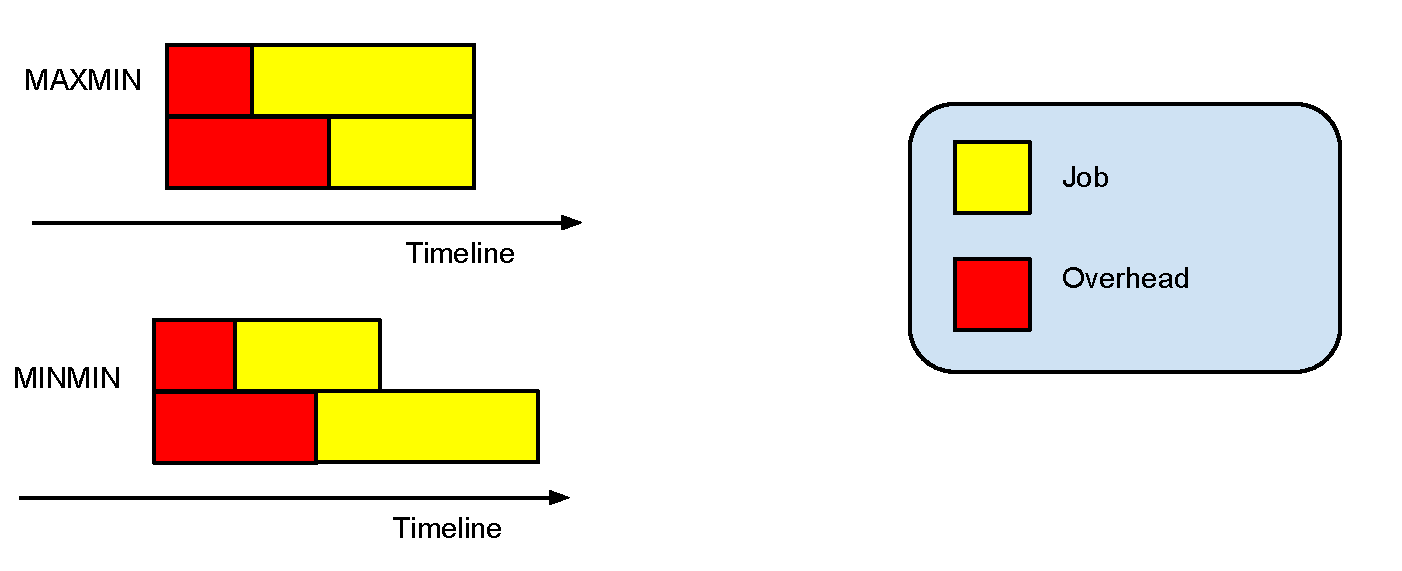
\includegraphics[width=1.0\linewidth]{figures/sensitivity/longest.pdf}
  \captionof{figure}{MAXMIN vs. MINMIN}
  \label{fig:sensitivity_longest}
\end{figure}
\emph{Breadth First} and \emph{Depth First}: Namely, the Breadth First (BFS) algorithm iterates the jobs at the same workflow level (or depth within a workflow directed acyclic graph) first while the Depth First (DFS) algorithm iterates the jobs at the deepest workflow level first. Intuitively speaking, we believe BFS performs better than DFS in terms of overhead robustness since BFS releases more jobs at the same workflow level for most scientific workflows as shown in Fig.~\ref{fig:sensitivity_shape}. Therefore, with enough jobs in queue, BFS can fully utilize the resources without wasting this overhead interval.  

\emph{Max Children First} and \emph{Min Children First}: The Max Children First (MAXCH) algorithm sorts all the unmapped jobs based on the number of children jobs that they have and assigns the jobs with most children jobs first. The Min Children First (MINCH) algorithm works in the opposite way and assigns the jobs with lest children jobs first. Similar to the case of BFS and DFS, we believe MAXCH should perform better than MINCH since MAXCH releases more jobs at the next level compared to MINCH and thus MAXCH can fully utilize the available resources. 

\begin{figure}[htb]
\centering
 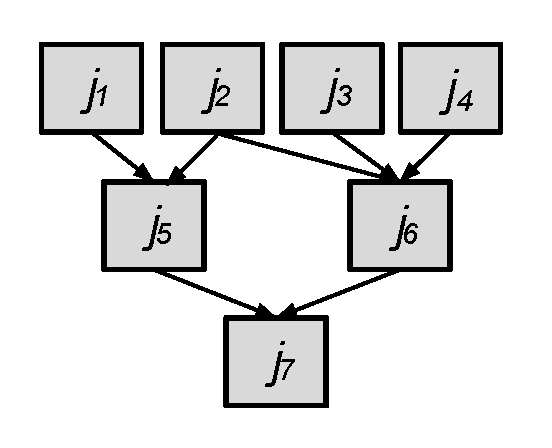
\includegraphics[width=0.5\linewidth]{figures/sensitivity/impact_factor.pdf}
  \captionof{figure}{Impact Factor}
  \label{fig:sensitivity_impact}
\end{figure}

\emph{Important First} and \emph{Unimportant First}: Here we propose a pair of Impact Factor based scheduling heuristics. The Important First (IFS) algorithm sorts all the unmapped jobs based on their \emph{Impact Factor} (IF) and assigns the jobs with the largest IF first while the Unimportant First (UIFS) algorithm assigns the jobs with the smallest IF first. 
The \textbf{Impact Factor} ($IF$) of a job $j_u$ is defined the same as Eq.~\ref{eq:imbalance_impact_factor}. 
For simplicity, we assume the $IF$ of a workflow exit job (e.g. $j_7$ in Fig.~\ref{fig:sensitivity_impact}) as 1.0. For instance, consider the workflow in Fig.~\ref{fig:sensitivity_impact}. $IF$ for $j_1$, $j_2$, $j_3$, and $j_4$ are computed as follows:

\begin{eqnarray}
	\displaystyle  
	&IF(j_7 )=1.0, IF(j_6 )=IF(j_5 )=IF(j_7 )/2=0.5\nonumber  \\
	&IF(j_1 )=IF(j_5)/2=0.25\nonumber \\
	&IF(j_2 )=IF(j_5 )/2+IF(j_6)/3=0.42\nonumber \\
	&IF(j_3 )=IF(j_4 )=IF(j_6 )/3=0.17\nonumber 
\end{eqnarray}
Thus, IFS algorithm should schedule $j_2$ first while UIFS algorithm should schedule $j_3$ or $j_4$ first. The intuition of Impact Factor is that we aim to measure the relative importance of a job to the entire graph. Intuitively speaking, tasks with larger impact factors should have more impacts on the remaining jobs compared to tasks with smaller impact factors. For example, a bottleneck usually has a larger IF since it controls the release of more jobs. 
Similar to the case of MAXCH and MINCH, we believe IFS has a better overhead robustness than UIFS since IFS releases more jobs at the next few levels compared to UIFS. 


%The idea of these overhead aware heuristics is we would like to improve the overhead robustness even when we are not able to precisely predict the duration of overheads. Instead, workflow overheads have common patterns, which can determine the relative performance of different heuristics. 
Table~\ref{tab:sensitivity_heuristics} summaries the heuristics and their potential overhead robustness. 
\begin{table}[H]
\caption{Scheduling Heuristics}
\begin{center}
  \begin{tabular}{ l|l|l}
    \hline
Heuristics & Overhead Robust & Overhead Unrobust \\ \hline
    Experiment 1 & MAXMIN & MINMIN \\ \hline
   Experiment 2 & BFS & DFS \\ \hline
 Experiment 3 & MAXCH & MINCH \\ \hline
Experiment 4 & IFS & UIFS\\
    \hline
  \end{tabular}
\label{tab:sensitivity_heuristics}
\end{center}
\end{table}

% Section
\subsection{Experiment Conditions}


The experiments presented hereafter evaluate the performance of the four pairs of heuristics mentioned ahead, which are widely used by workflow management systems. 

\begin{figure}[htb]
	\centering
	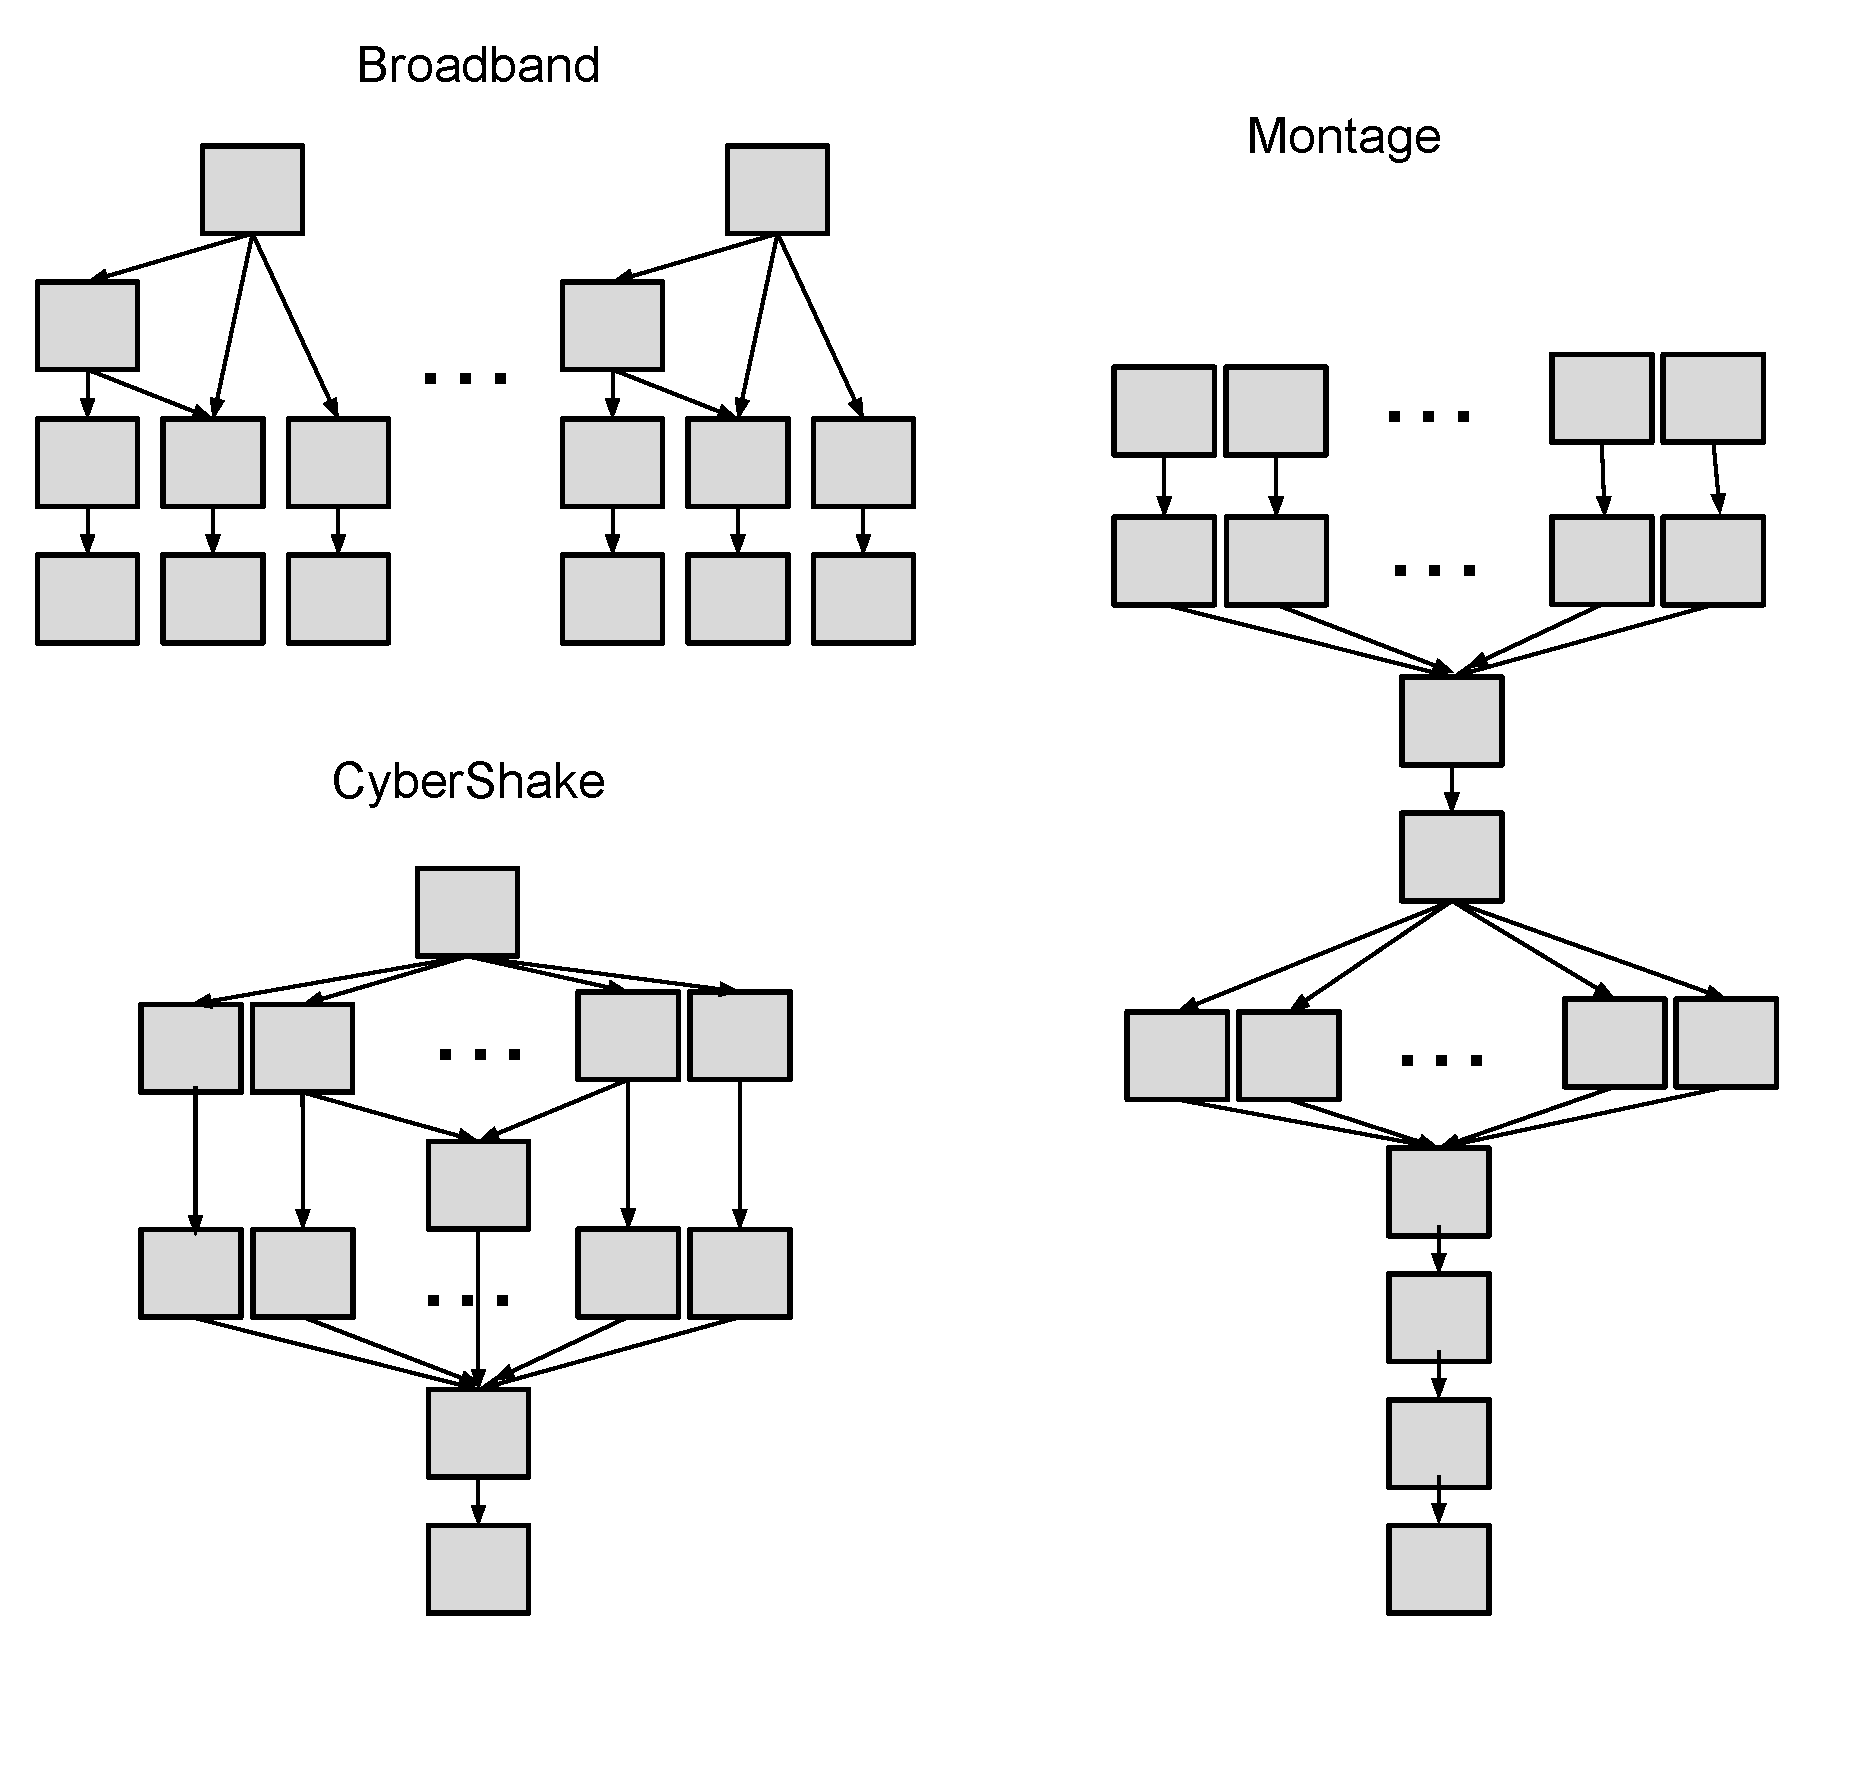
\includegraphics[width=1.0\linewidth]{figures/sensitivity/shape.pdf} 
	\caption{A simplified visualization of the Broadband workflow, the Montage workflow and the CyberShake workflow.}
	\label{fig:sensitivity_shape}
\end{figure}

We extended the WorkflowSim~\cite{Chen2012a} simulator with the overhead model to simulate a distributed environment where we could evaluate the overhead robustness of scheduling algorithms when varying the average overheads and throughput. As an initial attempt, we focus on the workflow engine delay ($d$) in this paper. The simulated computing platform is composed by 20 single core virtual machines (worker nodes), which is the quota per user of some typical distributed environments such as Amazon EC2~\cite{AmazonAWS} and FutureGrid~\cite{FutureGrid}. Each machine has 512MB of memory and the capacity to process 1,000 million instructions per second. 
%Task scheduling is data-aware, i.e. tasks are scheduled to resources which have the most input data available.
%WorkflowSim is a feature-rich toolkit to simulate workflow planning and execution. It provides runtime randomization and multiple task clustering methods that we need. 



Three workflows are used in the experiments: 
Broadband~\cite{Broadband} is an application that enables researchers to combine long-period deterministic seismograms with high-frequency stochastic seismograms. 
Montage~\cite{Sakellariou2010} is an astronomy application used to construct large image mosaics of the sky. CyberShake~\cite{Callaghan2008} is a seismology application that calculates Probabilistic Seismic Hazard curves for geographic sites in the Southern California region. All workflows are generated and varied using the WorkflowGenerator\footnote[1]{https://confluence.pegasus.isi.edu/display/pegasus/WorkflowGenerator}. Each workflow instance is composed by around 100 tasks and its workflow structure is presented in Fig.~\ref{fig:sensitivity_shape}. Runtime (average and task runtime distribution) and overhead (workflow engine delay and queue delay) information were collected from real traces production environments~\cite{Chen2011, Juve2013}, then used as input parameters for the simulations.

%We first collected runtime information  (i.e., average and distribution of task runtime) and overhead information (including workflow engine delay, queue delay and network bandwidth) from the real traces that were run on real environments before. 
%Part of runtime distribution and overhead information were shown in \cite{Juve2013} and \cite{Chen} respectively. 
%Then we input these parameters into WorkflowSim and run these workflows repeatedly until the variance is less than 5\% of the average workflow runtime. 



Four sets of experiments are conducted. Experiment 1 evaluates the relative robustness of MAXMIN and MINMIN by comparing the performance gain of the overhead robust heuristic (MAXMIN in this experiment) over the overhead unrobust heuristic (MINMIN), while varying the average interval of workflow engine ($d$) and throughput of workflow engine ($t$). Table~\ref{tab:sensitivity_heuristics} shows the heuristics compared in these experiments. Simulation results present a confidence level of 95\%. Thus, for values of \emph{Performance Gain} $> 0$, the overhead robust heuristics perform better than the respective overhead unrobust heuristics. Otherwise, the overhead robust heuristics perform poorer.
%We randomly select 20\% from LIGO workflow tasks and increase their task runtime by a factor of \emph{Ratio} to simulate the system variation in a production environment.




In these experiment sets, we vary the average throughput of workflow engine from 1 to 20 and we show the results of $t$=1, 5, 15, 20. The original throughput of workflow engine in these traces is 5 and a throughput that is larger than 20 does not influence the performance much since we have only 20 worker nodes in our experiments. We also vary the average interval of workflow engine from 0 to 100 seconds, which represents a typical range of workflow engine delay as shown in~\cite{Chen2011} and this range is able to show the difference of overhead robustness in these heuristics. 

\subsection{Results and Discussion}

\begin{figure}[!htb]
\centering
 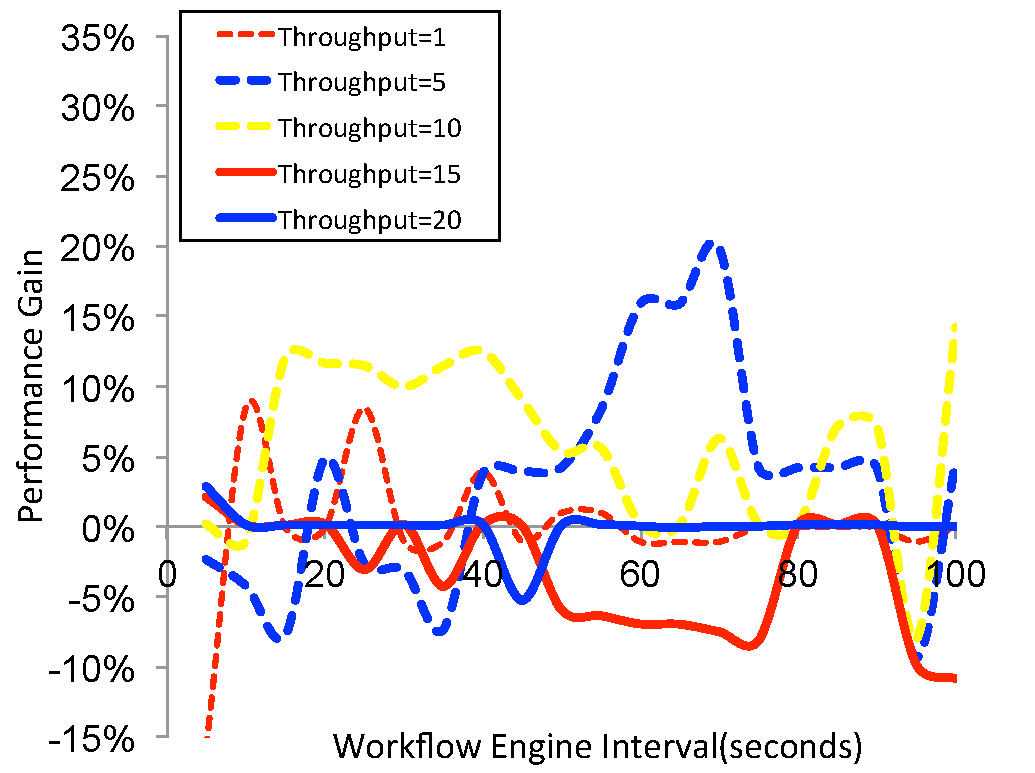
\includegraphics[width=0.9\linewidth]{figures/sensitivity/MAX-MIN-Broadband.pdf}
  \captionof{figure}{Broadband }
  \label{fig:sensitivity_MAX-MIN-Broadband}
\end{figure}

\begin{figure}[!htb]
\centering
 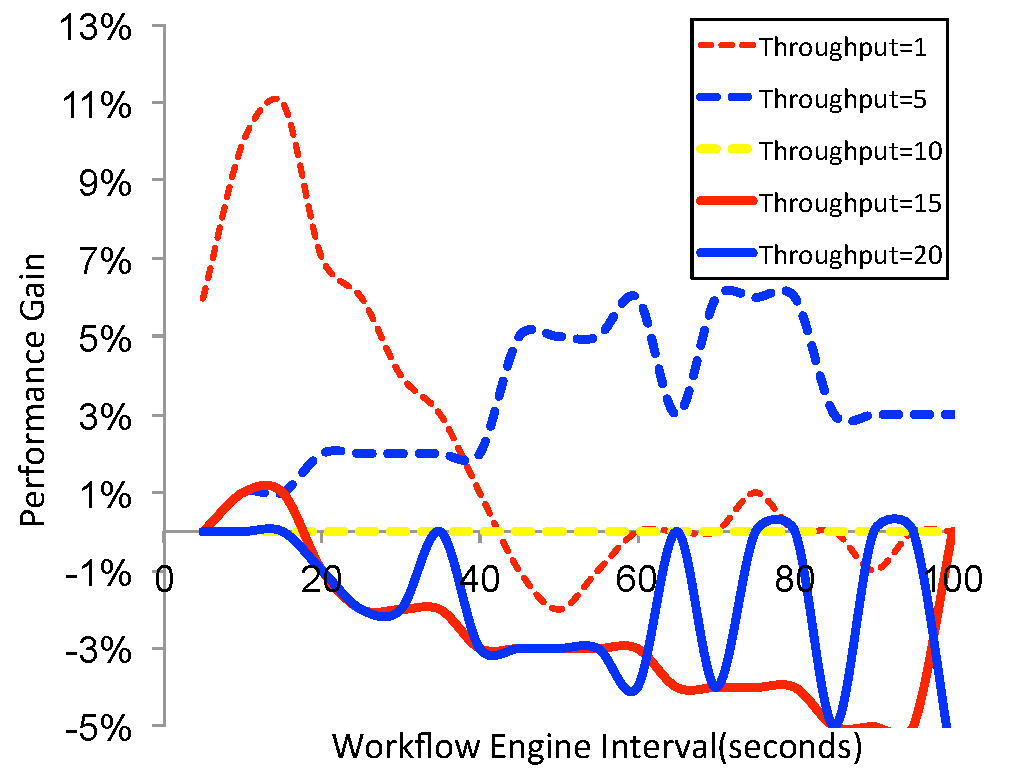
\includegraphics[width=0.9\linewidth]{figures/sensitivity/MAX-MIN-CyberShake.pdf}
  \captionof{figure}{CyberShake}
  \label{fig:sensitivity_MAX-MIN-CyberShake}
\end{figure}

\begin{figure}[!htb]
\centering
 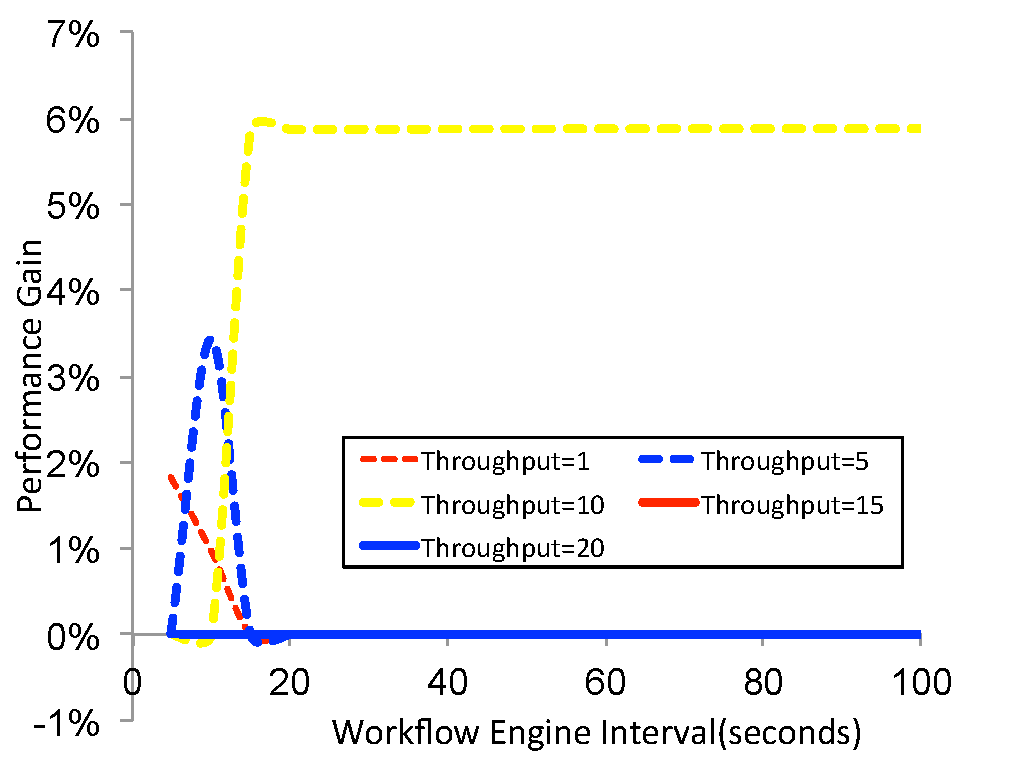
\includegraphics[width=0.9\linewidth]{figures/sensitivity/MAX-MIN-Montage.pdf}
  \captionof{figure}{Montage}
  \label{fig:sensitivity_MAX-MIN-Montage}
\end{figure}


Experiment 1: Fig.~\ref{fig:sensitivity_MAX-MIN-Broadband},~\ref{fig:sensitivity_MAX-MIN-CyberShake},~\ref{fig:sensitivity_MAX-MIN-Montage} show the  \emph{Performance Gain} of MAXMIN over MINMIN for the three workflows. We expected to see most  \emph{Performance Gain} $>0$ if MAXMIN is a overhead robust heuristic compared to MINMIN. However, except for the Montage workflow, the \emph{Performance Gain} is not significant for all of parameter settings, which concludes that MAXMIN is not globally overwhelming MINMIN in terms of overhead robustness. The reason we believe is that the  \emph{Performance Gain} in this comparison highly depends on the ratio of job runtime, workflow engine delay, number of resources and throughput of workflow engine. 

\begin{figure}[!htb]
\centering
 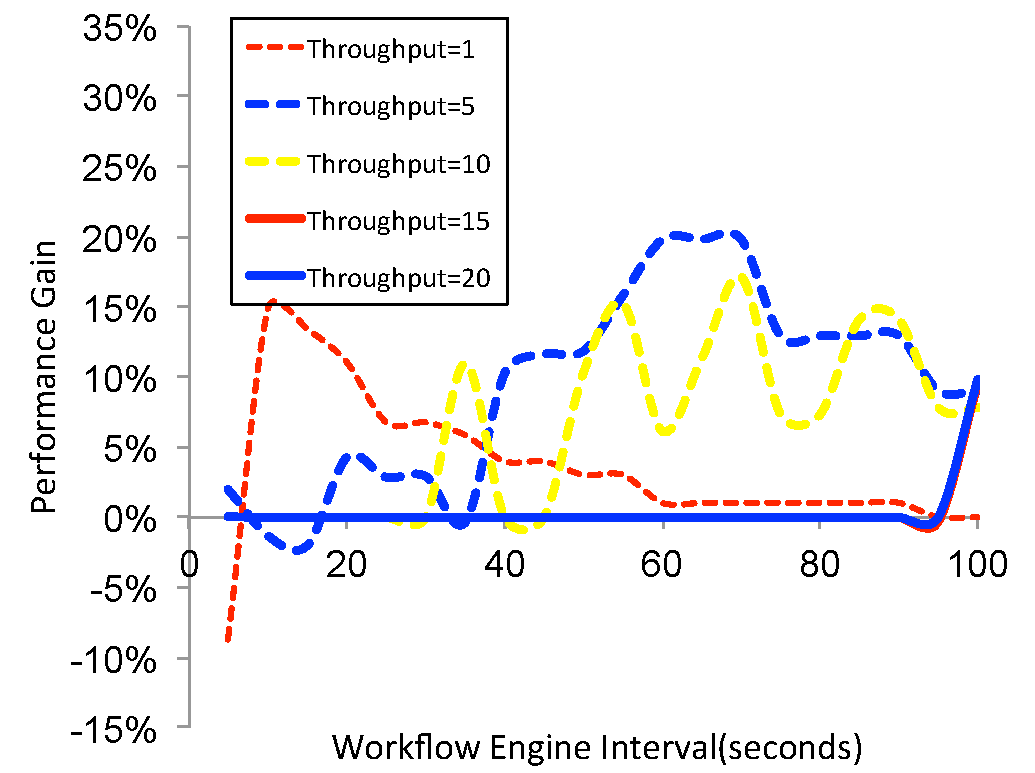
\includegraphics[width=0.9\linewidth]{figures/sensitivity/DFS-BFS-Broadband.pdf}
  \captionof{figure}{Broadband }
  \label{fig:sensitivity_DFS-BFS-Broadband}
\end{figure}

\begin{figure}[!htb]
\centering
 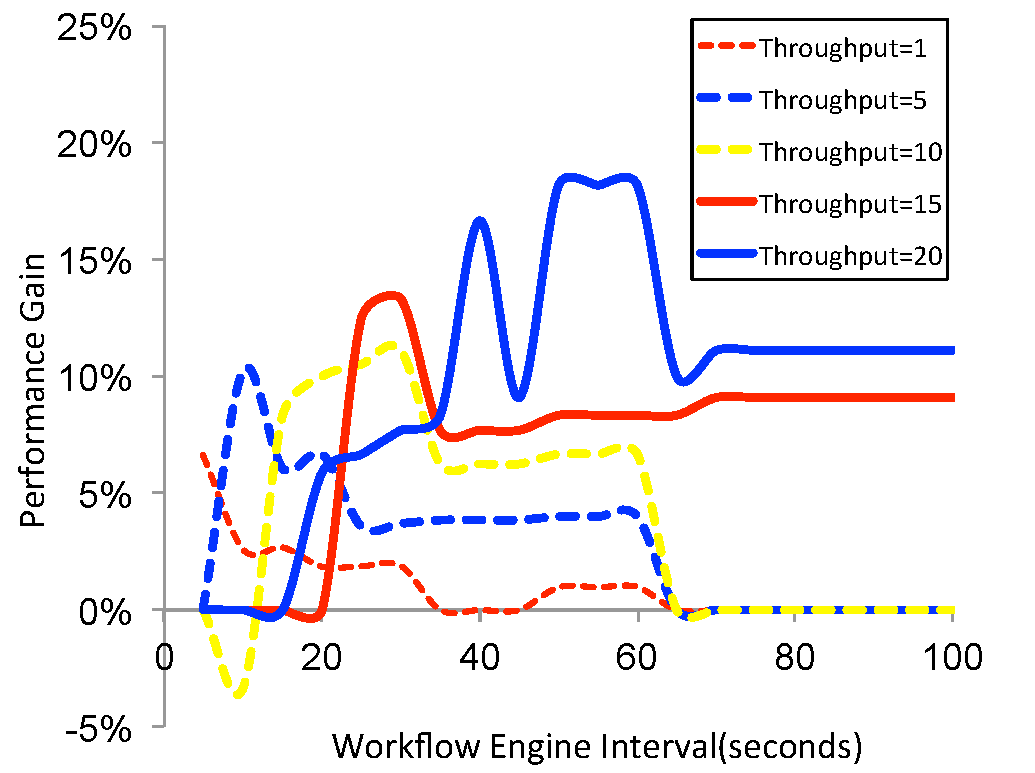
\includegraphics[width=0.9\linewidth]{figures/sensitivity/DFS-BFS-CyberShake.pdf}
  \captionof{figure}{CyberShake}
  \label{fig:sensitivity_DFS-BFS-CyberShake}
\end{figure}

\begin{figure}[!htb]
\centering
 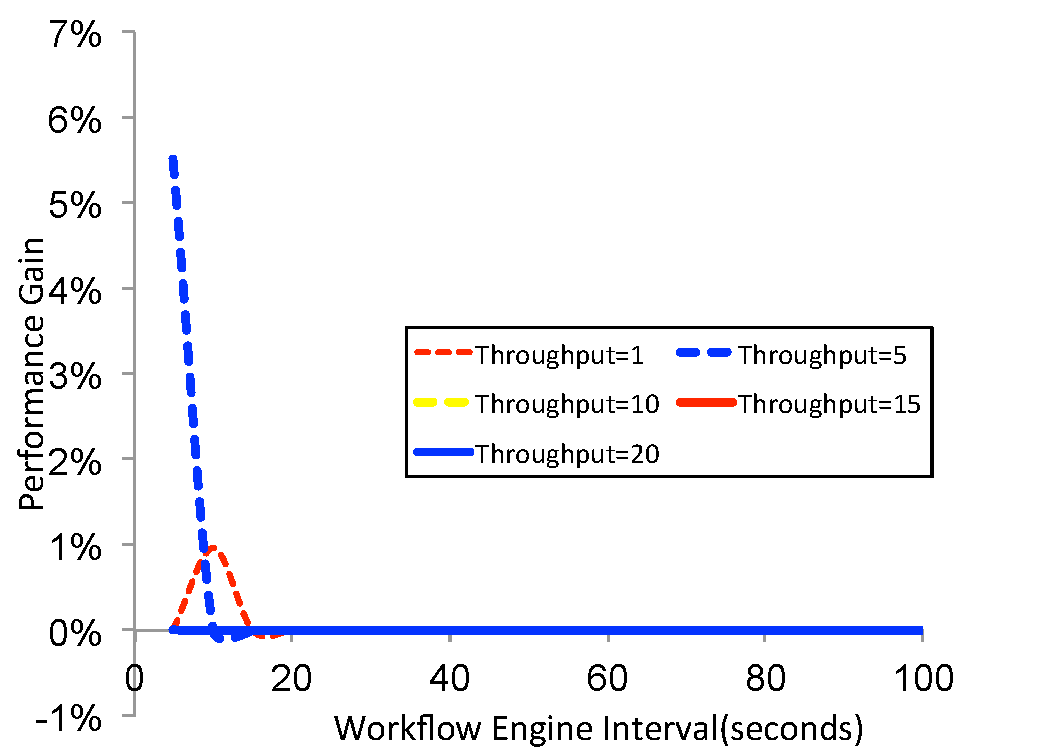
\includegraphics[width=0.9\linewidth]{figures/sensitivity/DFS-BFS-Montage.pdf}
  \captionof{figure}{Montage}
  \label{fig:sensitivity_DFS-BFS-Montage}
\end{figure}


Experiment 2: Fig.~\ref{fig:sensitivity_DFS-BFS-Broadband},~\ref{fig:sensitivity_DFS-BFS-CyberShake},~\ref{fig:sensitivity_DFS-BFS-Montage} show the \emph{Performance Gain} of BFS over DFS for the three workflows. We observe that most  \emph{Performance Gain} $>0$ and thus BFS performs better than DFS in terms of overhead robustness. What is more, Fig~\ref{fig:sensitivity_DFS-BFS-CyberShake} shows with the increase of average throughput, the \emph{Performance Gain} is more significant. We can also see that when the average throughput is high, the \emph{Performance Gain} increases with the average interval of workflow engine. This suggests us in a real environment with a large overhead, we should use BFS instead of DFS. 


\begin{figure}[!htb]
\centering
 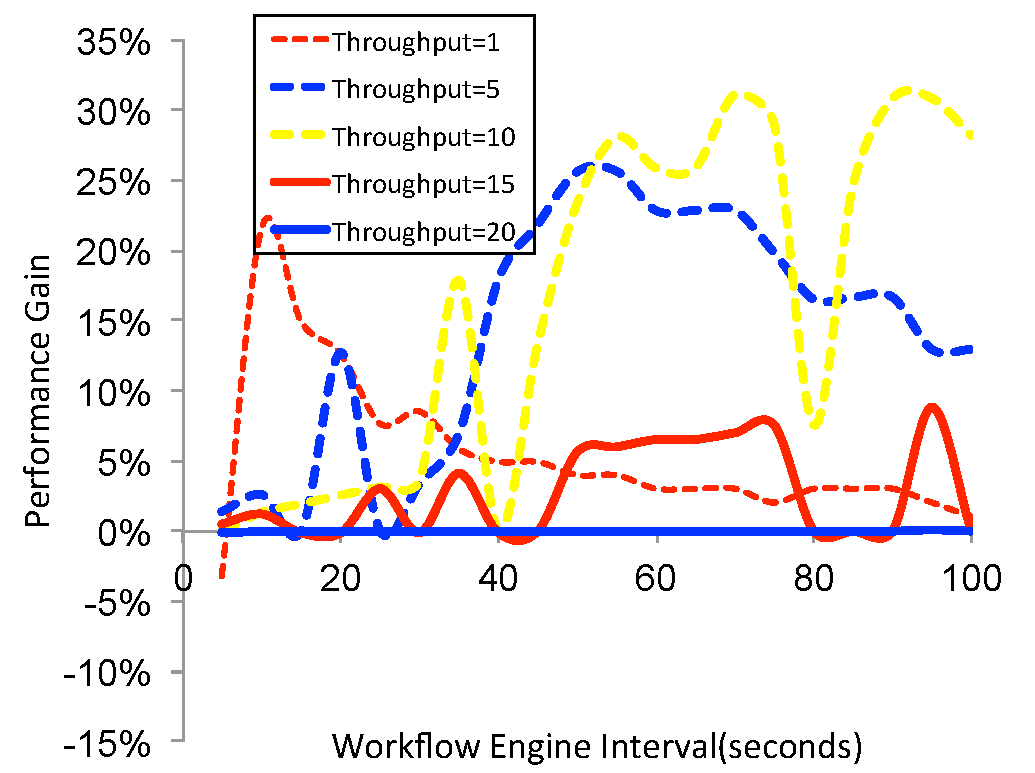
\includegraphics[width=0.9\linewidth]{figures/sensitivity/MINCH-MAXCH-Broadband.pdf}
  \captionof{figure}{Broadband }
  \label{fig:sensitivity_MINCH-MAXCH-Broadband}
\end{figure}

\begin{figure}[!htb]
\centering
 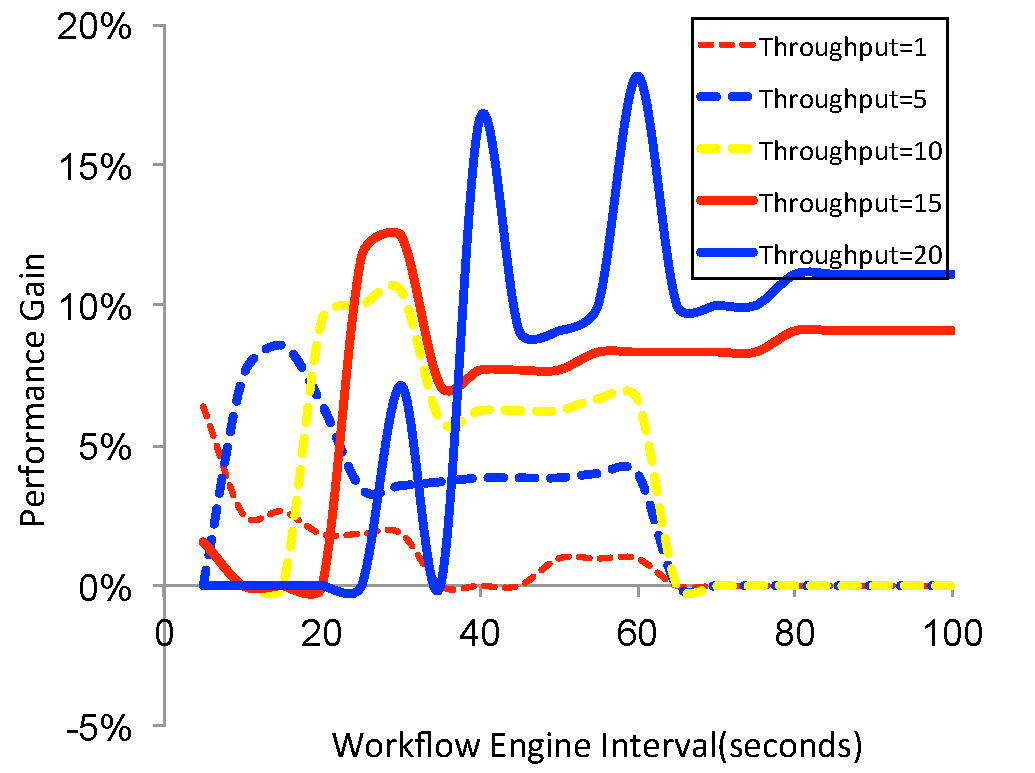
\includegraphics[width=0.9\linewidth]{figures/sensitivity/MINCH-MAXCH-CyberShake.pdf}
  \captionof{figure}{CyberShake}
  \label{fig:sensitivity_MINCH-MAXCH-CyberShake}
\end{figure}

\begin{figure}[!htb]
\centering
 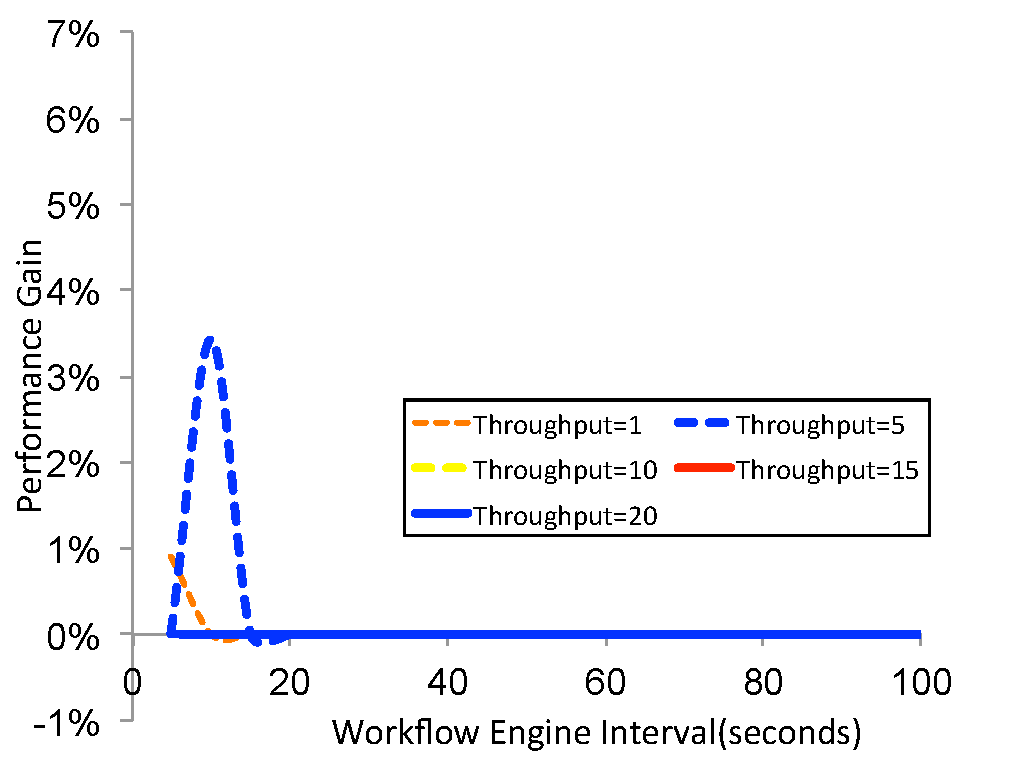
\includegraphics[width=0.9\linewidth]{figures/sensitivity/MINCH-MAXCH-Montage.pdf}
  \captionof{figure}{Montage}
  \label{fig:sensitivity_MINCH-MAXCH-Montage}
\end{figure}



Experiment 3: Fig.~\ref{fig:sensitivity_MINCH-MAXCH-Broadband},~\ref{fig:sensitivity_MINCH-MAXCH-CyberShake},~\ref{fig:sensitivity_MINCH-MAXCH-Montage} show the \emph{Performance Gain} of MAXCH over MINCH for the three workflows. We observe that most  \emph{Performance Gain} $>0$ and thus MAXCH performs better than MINCH in terms of overhead robustness, which is similar to Experiment 2. Comparing Fig.~\ref{fig:sensitivity_DFS-BFS-Broadband} and Fig.~\ref{fig:sensitivity_MINCH-MAXCH-Broadband} we can see the \emph{Performance Gain} of MAXCH over MINCH is more significant (30\%) than that of BFS over DFS (20\%).  
\begin{figure}[!htb]
\centering
 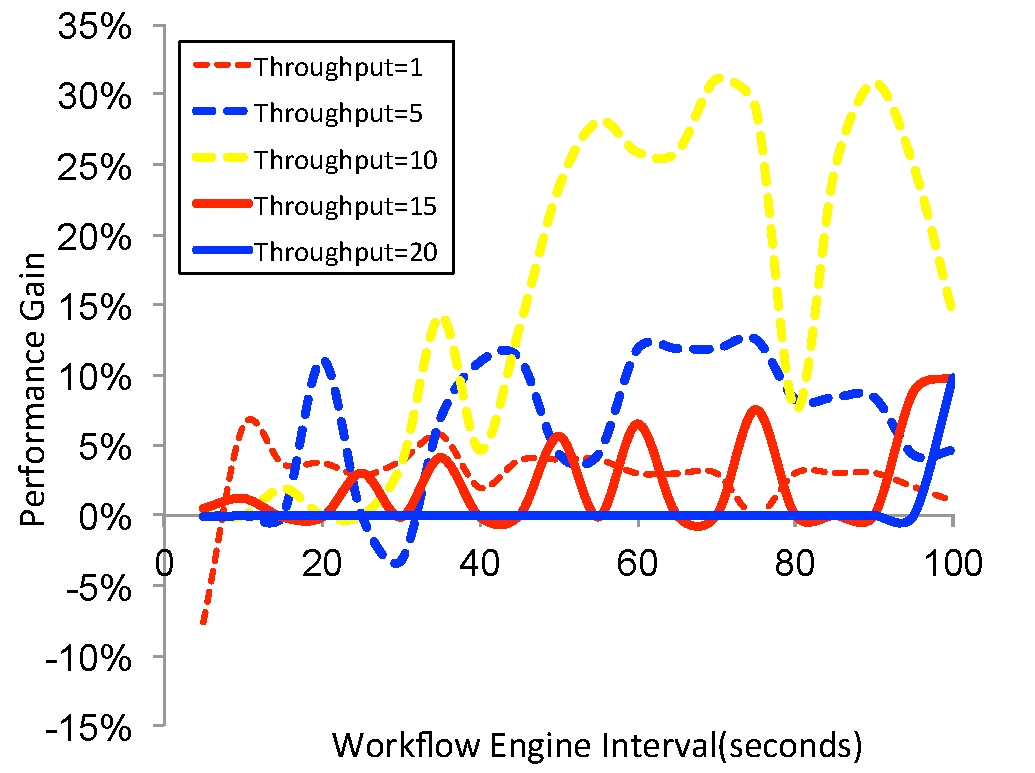
\includegraphics[width=0.9\linewidth]{figures/sensitivity/UIFS-IFS-Broadband.pdf}
  \captionof{figure}{Broadband }
  \label{fig:sensitivity_UIFS-IFS-Broadband}
\end{figure}

\begin{figure}[!htb]
\centering
 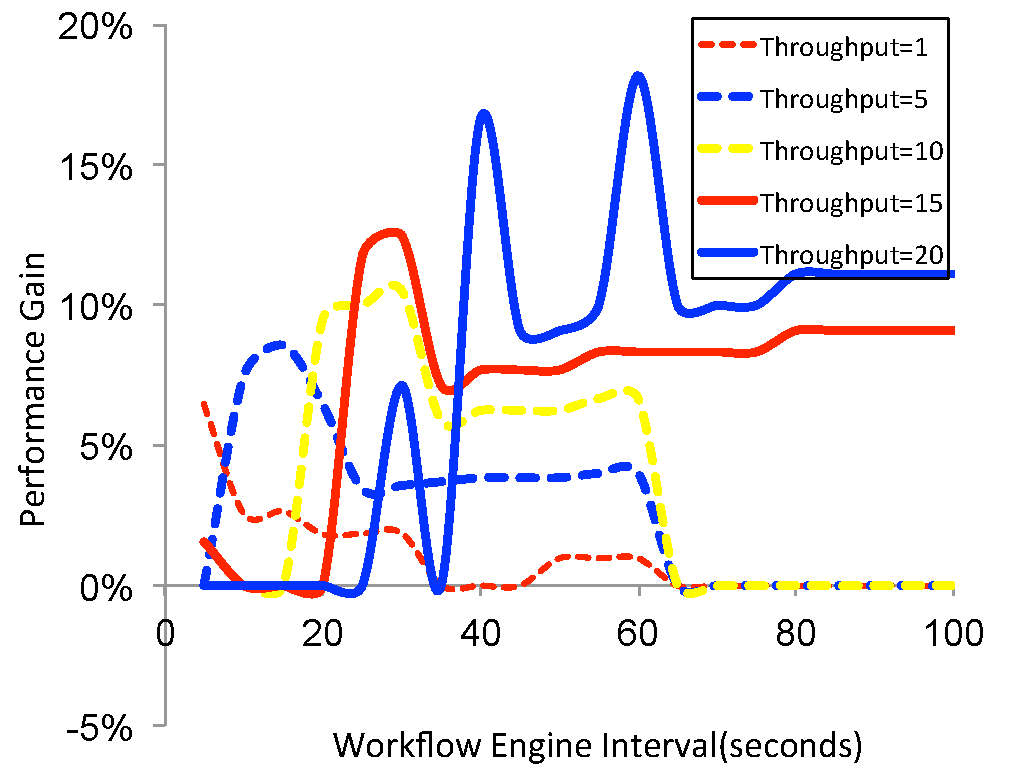
\includegraphics[width=0.9\linewidth]{figures/sensitivity/UIFS-IFS-CyberShake.pdf}
  \captionof{figure}{CyberShake}
  \label{fig:sensitivity_UIFS-IFS-CyberShake}
\end{figure}

\begin{figure}[!htb]
\centering
 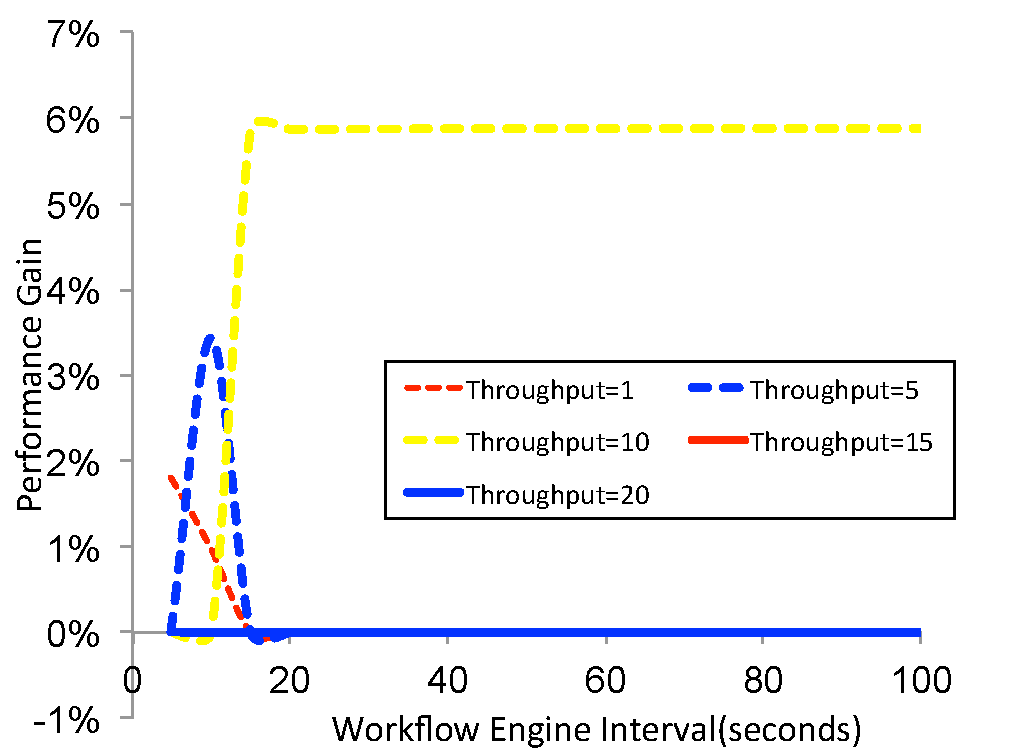
\includegraphics[width=0.9\linewidth]{figures/sensitivity/UIFS-IFS-Montage.pdf}
  \captionof{figure}{Montage}
  \label{fig:sensitivity_UIFS-IFS-Montage}
\end{figure}
Experiment 4: Fig.~\ref{fig:sensitivity_UIFS-IFS-Broadband},~\ref{fig:sensitivity_UIFS-IFS-CyberShake},~\ref{fig:sensitivity_UIFS-IFS-Montage} show the \emph{Performance Gain} of IFS over UIFS for the three workflows. We observe that most  \emph{Performance Gain} $>0$ and thus IFS performs better than UIFS in terms of overhead robustness, which is similar to Experiment 3. The reason is that for these workflows, IF based heuristics can produce similar schedule as the heuristics based on the number of children. Most of the workflows used in this paper is not irregular enough and thus we are not able to show the difference of IF based heuristics and the heuristics based on the number of children. 

